%----------------------------------------------------------------------------------------
%   PACKAGES AND OTHER DOCUMENT CONFIGURATIONS
%----------------------------------------------------------------------------------------

\documentclass[11pt]{article}

\usepackage[english]{babel}
\usepackage[utf8x]{inputenc}
\usepackage{amsmath}
\usepackage{graphicx}
\usepackage{csquotes}
\usepackage{hyperref}
\usepackage{fancyvrb}
\usepackage{url}
\usepackage[a4paper, total={6in, 8in}]{geometry}
\usepackage[colorinlistoftodos]{todonotes}

\setlength{\parskip}{0.4em}

%----------------------------------------------------------------------------------------
%   HEADING
%----------------------------------------------------------------------------------------

\newcommand{\BigO}[1]{\ensuremath{\operatorname{O}\left(#1\right)}}

\title{\textsc{Software Engineering}\\Week IV~- Software Architecture}
\author{Lawrence Jones \{lmj112\} \  Alice Sibold \{as4712\} \\
        Joshua Coutinho \{jrc12\}}

\date{}
\begin{document}
\maketitle

%----------------------------------------------------------------------------------------
%   BODY
%----------------------------------------------------------------------------------------

\textit{Our discussion about how to frame this architecture can be seen in our
collaborative scoping document\cite{scoping}, where we detailed an overview of
each architectural tier.}

\subsection*{What do you think is most important to show in describing software
architecture of this system?}

The diverse technical background of stackholders means it is crucial to describe
the architecture in ways that can be suitable for each
stakeholder~\cite{rozanski}, rather than relying on one giant model for all.\\

Customers will be most interested in scenario views, covering their use cases,
such as that provided in Figure~\ref{fig:scenario}. This gives them confidence
in the system by communicating how it will work in real-world instances.\\

Management at the RAH will be more interested in a functional diagram. This maps
out major parts of the system, and shows what features there are and how they
connect (see Figure~\ref{fig:functional}). This high-level view of the system
allows stakeholders - while having limited technical knowledge - to evaluate
whether the desired functionality of the system is maintained and additional
requirements satisfied.\\

There are no standards for architectural diagrams; rather, they are specific to
teams and organisations and evolve over time. As Brown mentions in his appeal
for conventionalised NoUML architectural diagrams~\cite{brown}, the single most
important aspect is to have clear and consistent conventions understood by all
team members (e.g. colour coding, legend, etc.).

The main challenge that the RAH faces for its reservation system is
availability. The most effective way to ensure availability~\cite{bot} is to
design a scalabale solution~\cite{prom} that is intended to handle failure at
different levels. Solutions should also automatically grow/shrink the number of
running instances in response to traffic - high availability with minimal
maintainence. \\

The most important architectural aid then, is one that is approachable by the
greatest number of stakeholders, facilitating the use of architecture as a
communication tool across the team. The selection of such a tool is dependent on
the stakeholders of the project, and can be determined by the collection of
stakeholders for whom it can provide most use.

%----------------------------------------------------------------------------------------
%   BIBLIOGRAPHY
%----------------------------------------------------------------------------------------

\begin{thebibliography}{99}
\bibitem{rozanski} Rozanski and Woods - \emph{Applying Viewpoints and Views to
  Software Architecture} \\
  \path{http://www.viewpoints-and-perspectives.info/vpandp/wp-content/themes/secondedition/doc/VPandV_WhitePaper.pdf}

\bibitem{brown} Brown - \emph{Agile Software Architecture Sketches and NoUML} \\
  \path{http://www.infoq.com/articles/agile-software-architecture-sketches-NoUML}

\bibitem{prom} BBC News - \emph{Over 110,000 tickets sold as booking opens for
  2014 BBC Proms} \\
  \path{http://www.bbc.co.uk/mediacentre/latestnews/2014/proms-tickets}

\bibitem{bot} Flyn - \emph{The Bot Wars: why you can never buy concert tickets
  online} \\
  \path{http://www.newstatesman.com/economics/2013/08/bot-wars-why-you-can-never-buy-concert-tickets-online}

\bibitem{scoping} Team Scoping Document - \emph{Lightweight overview of
  architectural tiers} \\
  \path{https://paper.dropbox.com/doc/SoftEng-Albert-Hall-Tickets-IkMoYl43HuXhywG3f0Nxl}
\end{thebibliography}

\newpage

%----------------------------------------------------------------------------------------
%   DIAGRAMS
%----------------------------------------------------------------------------------------

\subsection*{Diagrams}
\begin{center}

\begin{figure}[h]
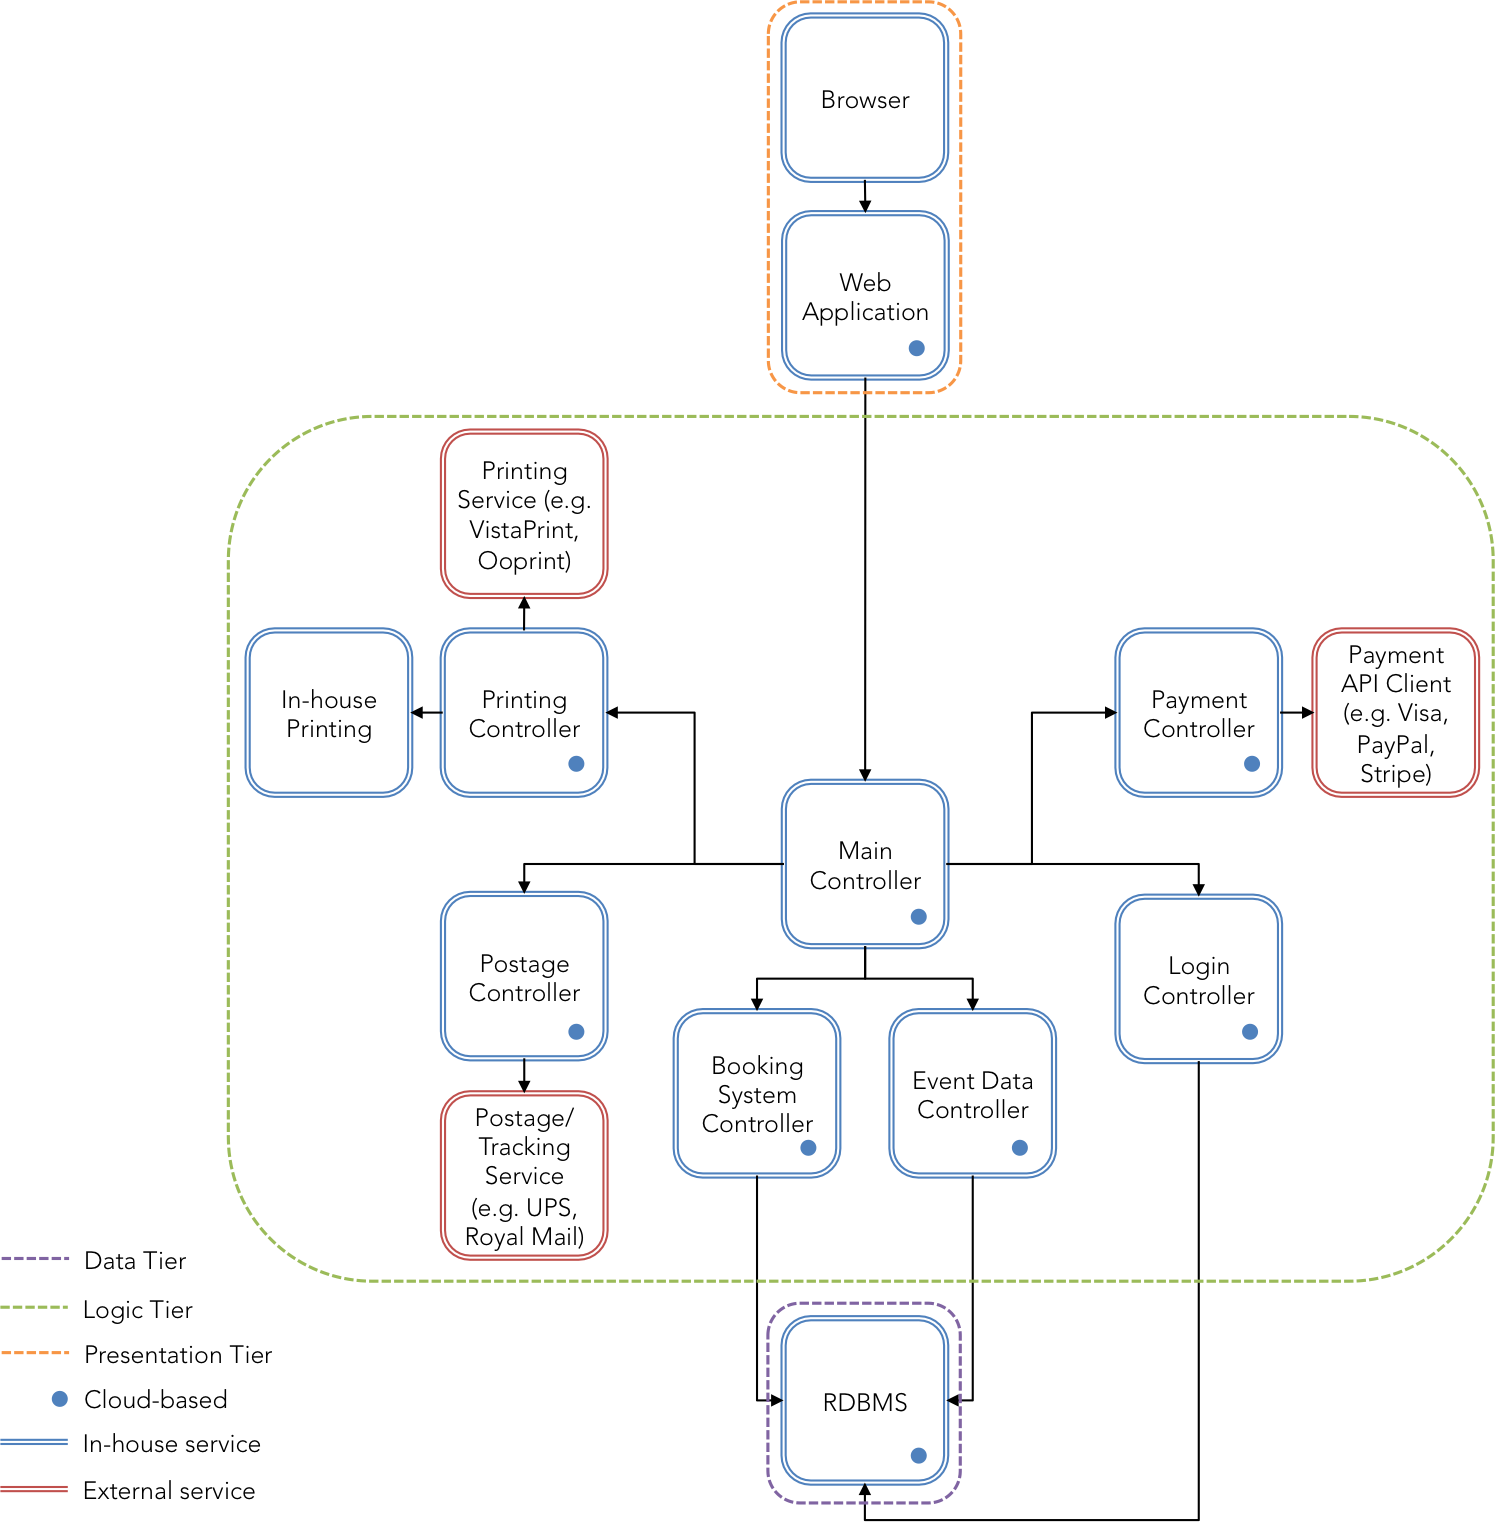
\includegraphics[width=14.5cm]{lib/res/Functional.png}
\caption{Functional Diagram}
\label{fig:functional}
\end{figure}

\begin{figure}[h]
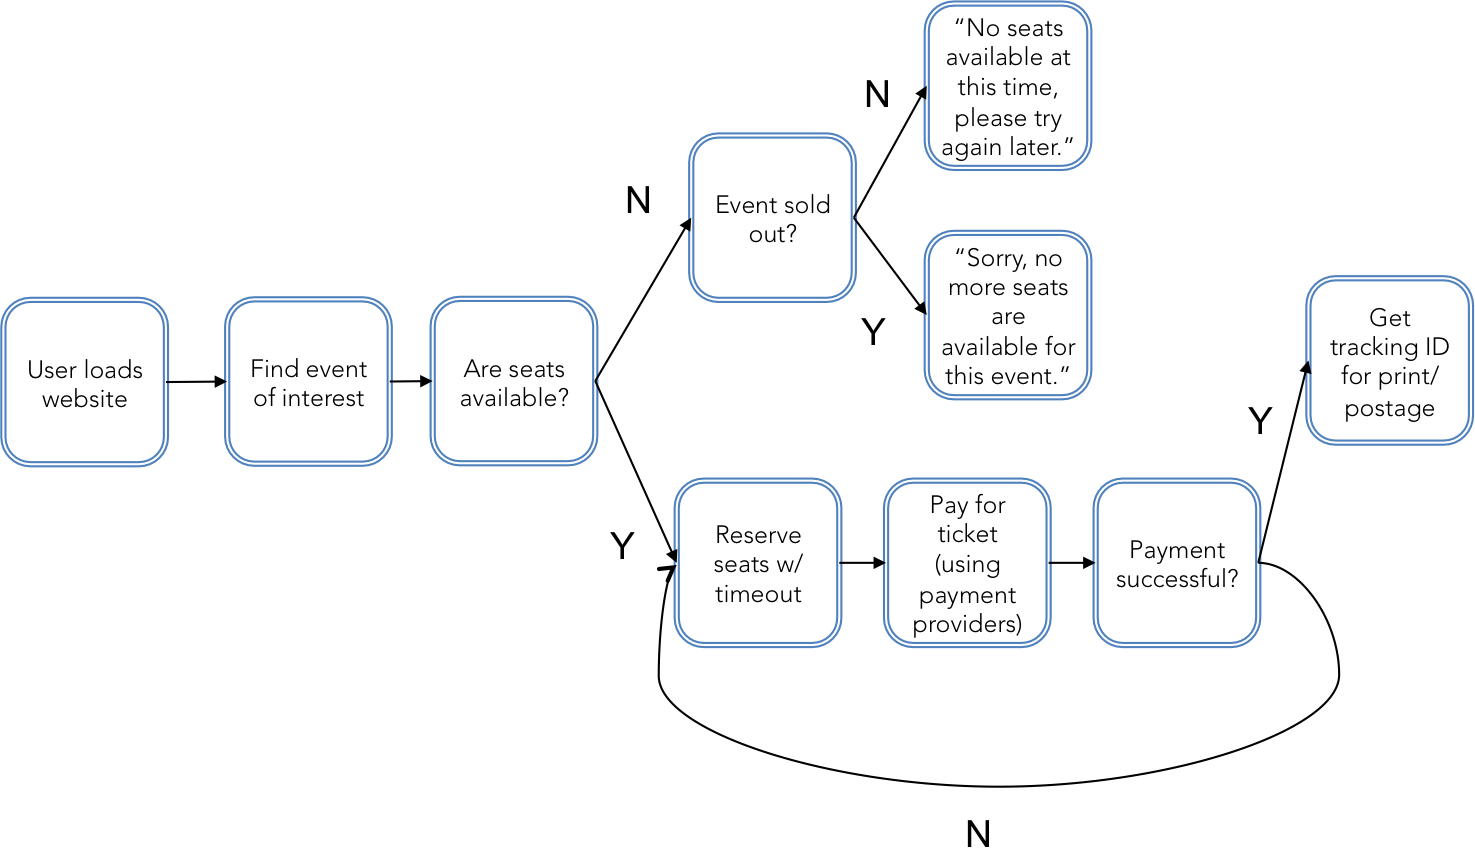
\includegraphics[width=15cm]{lib/res/Scenario.png}
\caption{Scenario Diagram}
\label{fig:scenario}
\end{figure}

\end{center}

\end{document}
